\documentclass[twoside]{book}

% Packages required by doxygen
\usepackage{calc}
\usepackage{doxygen}
\usepackage{graphicx}
\usepackage[utf8]{inputenc}
\usepackage{makeidx}
\usepackage{multicol}
\usepackage{multirow}
\usepackage{textcomp}
\usepackage[table]{xcolor}

% Font selection
\usepackage[T1]{fontenc}
\usepackage{mathptmx}
\usepackage[scaled=.90]{helvet}
\usepackage{courier}
\usepackage{amssymb}
\usepackage{sectsty}
\renewcommand{\familydefault}{\sfdefault}
\allsectionsfont{%
  \fontseries{bc}\selectfont%
  \color{darkgray}%
}
\renewcommand{\DoxyLabelFont}{%
  \fontseries{bc}\selectfont%
  \color{darkgray}%
}

% Page & text layout
\usepackage{geometry}
\geometry{%
  a4paper,%
  top=2.5cm,%
  bottom=2.5cm,%
  left=2.5cm,%
  right=2.5cm%
}
\tolerance=750
\hfuzz=15pt
\hbadness=750
\setlength{\emergencystretch}{15pt}
\setlength{\parindent}{0cm}
\setlength{\parskip}{0.2cm}
\makeatletter
\renewcommand{\paragraph}{%
  \@startsection{paragraph}{4}{0ex}{-1.0ex}{1.0ex}{%
    \normalfont\normalsize\bfseries\SS@parafont%
  }%
}
\renewcommand{\subparagraph}{%
  \@startsection{subparagraph}{5}{0ex}{-1.0ex}{1.0ex}{%
    \normalfont\normalsize\bfseries\SS@subparafont%
  }%
}
\makeatother

% Headers & footers
\usepackage{fancyhdr}
\pagestyle{fancyplain}
\fancyhead[LE]{\fancyplain{}{\bfseries\thepage}}
\fancyhead[CE]{\fancyplain{}{}}
\fancyhead[RE]{\fancyplain{}{\bfseries\leftmark}}
\fancyhead[LO]{\fancyplain{}{\bfseries\rightmark}}
\fancyhead[CO]{\fancyplain{}{}}
\fancyhead[RO]{\fancyplain{}{\bfseries\thepage}}
\fancyfoot[LE]{\fancyplain{}{}}
\fancyfoot[CE]{\fancyplain{}{}}
\fancyfoot[RE]{\fancyplain{}{\bfseries\scriptsize Generated on Sat Feb 1 2014 21\-:26\-:15 for Lib\-Timer by Doxygen }}
\fancyfoot[LO]{\fancyplain{}{\bfseries\scriptsize Generated on Sat Feb 1 2014 21\-:26\-:15 for Lib\-Timer by Doxygen }}
\fancyfoot[CO]{\fancyplain{}{}}
\fancyfoot[RO]{\fancyplain{}{}}
\renewcommand{\footrulewidth}{0.4pt}
\renewcommand{\chaptermark}[1]{%
  \markboth{#1}{}%
}
\renewcommand{\sectionmark}[1]{%
  \markright{\thesection\ #1}%
}

% Indices & bibliography
\usepackage{natbib}
\usepackage[titles]{tocloft}
\setcounter{tocdepth}{3}
\setcounter{secnumdepth}{5}
\makeindex

% Hyperlinks (required, but should be loaded last)
\usepackage{ifpdf}
\ifpdf
  \usepackage[pdftex,pagebackref=true]{hyperref}
\else
  \usepackage[ps2pdf,pagebackref=true]{hyperref}
\fi
\hypersetup{%
  colorlinks=true,%
  linkcolor=blue,%
  citecolor=blue,%
  unicode%
}

% Custom commands
\newcommand{\clearemptydoublepage}{%
  \newpage{\pagestyle{empty}\cleardoublepage}%
}


%===== C O N T E N T S =====

\begin{document}

% Titlepage & ToC
\hypersetup{pageanchor=false}
\pagenumbering{roman}
\begin{titlepage}
\vspace*{7cm}
\begin{center}%
{\Large Lib\-Timer }\\
\vspace*{1cm}
{\large Generated by Doxygen 1.8.6}\\
\vspace*{0.5cm}
{\small Sat Feb 1 2014 21:26:15}\\
\end{center}
\end{titlepage}
\clearemptydoublepage
\tableofcontents
\clearemptydoublepage
\pagenumbering{arabic}
\hypersetup{pageanchor=true}

%--- Begin generated contents ---
\chapter{Lib\-Timer -\/ library for high performance timing}
\label{index}\hypertarget{index}{}This library can be used to time pieces of code or entire commands. 
\chapter{Hierarchical Index}
\section{Class Hierarchy}
This inheritance list is sorted roughly, but not completely, alphabetically\-:\begin{DoxyCompactList}
\item \contentsline{section}{Base\-Timer}{\pageref{class_base_timer}}{}
\begin{DoxyCompactList}
\item \contentsline{section}{Exec\-Timer}{\pageref{class_exec_timer}}{}
\end{DoxyCompactList}
\end{DoxyCompactList}

\chapter{Class Index}
\section{Class List}
Here are the classes, structs, unions and interfaces with brief descriptions\-:\begin{DoxyCompactList}
\item\contentsline{section}{\hyperlink{class_base_timer}{Base\-Timer} }{\pageref{class_base_timer}}{}
\item\contentsline{section}{\hyperlink{class_exec_timer}{Exec\-Timer} }{\pageref{class_exec_timer}}{}
\end{DoxyCompactList}

\chapter{Class Documentation}
\hypertarget{class_base_timer}{\section{Base\-Timer Class Reference}
\label{class_base_timer}\index{Base\-Timer@{Base\-Timer}}
}


{\ttfamily \#include $<$basetimer.\-h$>$}

Inheritance diagram for Base\-Timer\-:\begin{figure}[H]
\begin{center}
\leavevmode
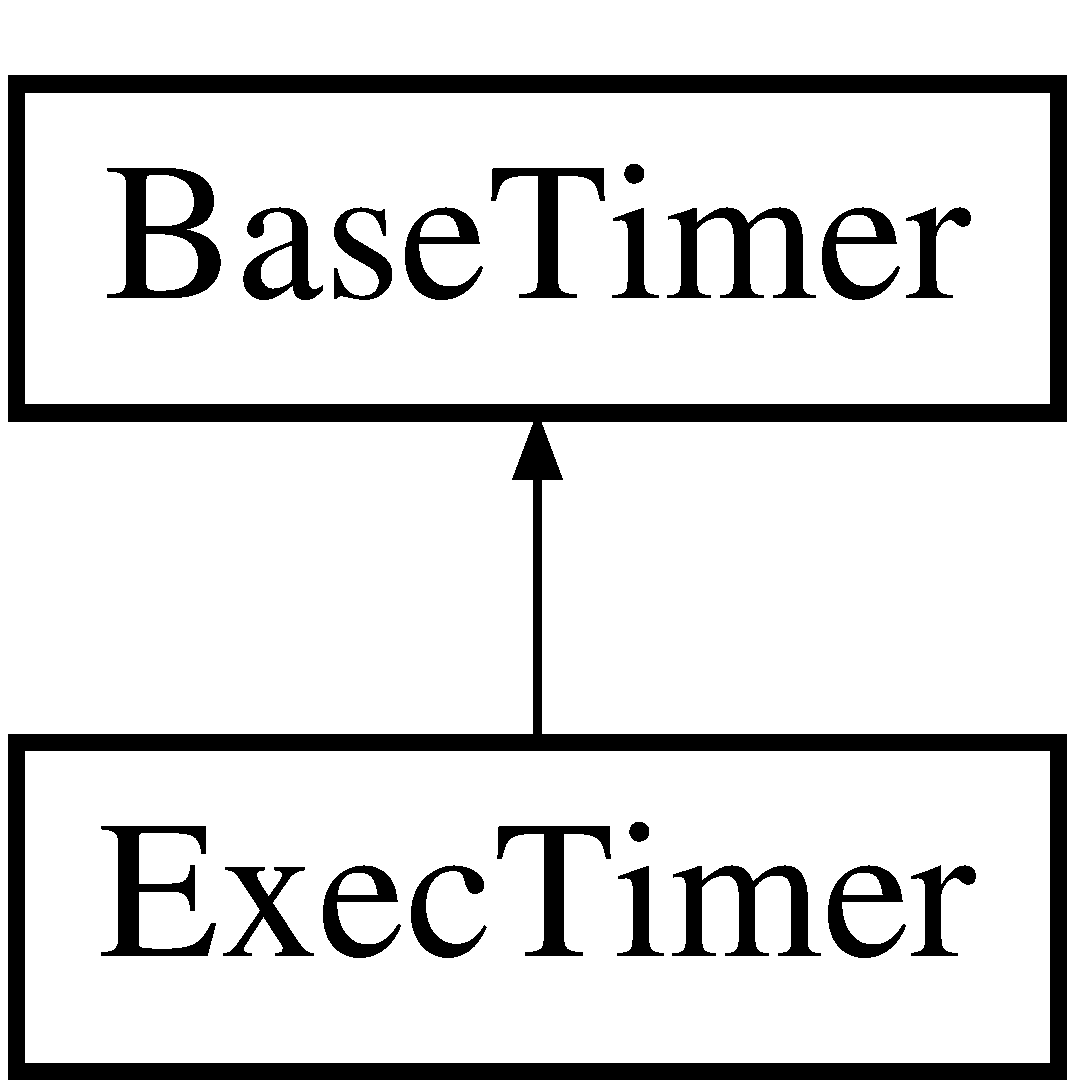
\includegraphics[height=2.000000cm]{class_base_timer}
\end{center}
\end{figure}
\subsection*{Public Member Functions}
\begin{DoxyCompactItemize}
\item 
\hyperlink{class_base_timer_a1a03059373391ed51149d21182db8fa4}{Base\-Timer} ()
\item 
bool \hyperlink{class_base_timer_ad1a4dc398bd40b4c19bb9f5687358e94}{start} ()
\item 
bool \hyperlink{class_base_timer_ae0ad1c2cc4decd0e03149eb514edcaa6}{stop} ()
\item 
void \hyperlink{class_base_timer_a91b31d11717b29761f38e8ea43d39063}{reset} ()
\item 
unsigned long long \hyperlink{class_base_timer_ad5d4815b9a6ca8042316fccaef433647}{elapsed\-Micro\-Seconds} ()
\item 
unsigned long long \hyperlink{class_base_timer_a0d2fa9af0f004932607be09748265db8}{elapsed\-Milli\-Seconds} ()
\item 
double \hyperlink{class_base_timer_aaa9c1ff59a32c340bf0244df37ad5a86}{elapsed\-Seconds} ()
\item 
void \hyperlink{class_base_timer_a078e5499b51d151695649dc333efdde6}{store} (std\-::string label)
\item 
bool \hyperlink{class_base_timer_a97047266ceaae87631d025957d3dffc8}{save} (std\-::string filename)
\end{DoxyCompactItemize}


\subsection{Detailed Description}
This is the main class of the library. This class is responsible for all the timing. It uses the High-\/\-Performance counters of Windows. 

\subsection{Constructor \& Destructor Documentation}
\hypertarget{class_base_timer_a1a03059373391ed51149d21182db8fa4}{\index{Base\-Timer@{Base\-Timer}!Base\-Timer@{Base\-Timer}}
\index{Base\-Timer@{Base\-Timer}!BaseTimer@{Base\-Timer}}
\subsubsection[{Base\-Timer}]{\setlength{\rightskip}{0pt plus 5cm}Base\-Timer\-::\-Base\-Timer (
\begin{DoxyParamCaption}
{}
\end{DoxyParamCaption}
)}}\label{class_base_timer_a1a03059373391ed51149d21182db8fa4}
The main constructor of the \hyperlink{class_base_timer}{Base\-Timer} class. This initializes everything to zero. 

\subsection{Member Function Documentation}
\hypertarget{class_base_timer_ad5d4815b9a6ca8042316fccaef433647}{\index{Base\-Timer@{Base\-Timer}!elapsed\-Micro\-Seconds@{elapsed\-Micro\-Seconds}}
\index{elapsed\-Micro\-Seconds@{elapsed\-Micro\-Seconds}!BaseTimer@{Base\-Timer}}
\subsubsection[{elapsed\-Micro\-Seconds}]{\setlength{\rightskip}{0pt plus 5cm}unsigned long long Base\-Timer\-::elapsed\-Micro\-Seconds (
\begin{DoxyParamCaption}
{}
\end{DoxyParamCaption}
)}}\label{class_base_timer_ad5d4815b9a6ca8042316fccaef433647}
This function will calculate the duration of the last timing. \begin{DoxyReturn}{Returns}
The time in microseconds between the \hyperlink{class_base_timer_ad1a4dc398bd40b4c19bb9f5687358e94}{start()} and the \hyperlink{class_base_timer_ae0ad1c2cc4decd0e03149eb514edcaa6}{stop()} 
\end{DoxyReturn}
\hypertarget{class_base_timer_a0d2fa9af0f004932607be09748265db8}{\index{Base\-Timer@{Base\-Timer}!elapsed\-Milli\-Seconds@{elapsed\-Milli\-Seconds}}
\index{elapsed\-Milli\-Seconds@{elapsed\-Milli\-Seconds}!BaseTimer@{Base\-Timer}}
\subsubsection[{elapsed\-Milli\-Seconds}]{\setlength{\rightskip}{0pt plus 5cm}unsigned long long Base\-Timer\-::elapsed\-Milli\-Seconds (
\begin{DoxyParamCaption}
{}
\end{DoxyParamCaption}
)}}\label{class_base_timer_a0d2fa9af0f004932607be09748265db8}
This function will calculate the duration of the last timing. \begin{DoxyReturn}{Returns}
The time in milliseconds between the \hyperlink{class_base_timer_ad1a4dc398bd40b4c19bb9f5687358e94}{start()} and the \hyperlink{class_base_timer_ae0ad1c2cc4decd0e03149eb514edcaa6}{stop()} 
\end{DoxyReturn}
\hypertarget{class_base_timer_aaa9c1ff59a32c340bf0244df37ad5a86}{\index{Base\-Timer@{Base\-Timer}!elapsed\-Seconds@{elapsed\-Seconds}}
\index{elapsed\-Seconds@{elapsed\-Seconds}!BaseTimer@{Base\-Timer}}
\subsubsection[{elapsed\-Seconds}]{\setlength{\rightskip}{0pt plus 5cm}double Base\-Timer\-::elapsed\-Seconds (
\begin{DoxyParamCaption}
{}
\end{DoxyParamCaption}
)}}\label{class_base_timer_aaa9c1ff59a32c340bf0244df37ad5a86}
This function will calculate the duration of the last timing. \begin{DoxyReturn}{Returns}
The time in seconds between the \hyperlink{class_base_timer_ad1a4dc398bd40b4c19bb9f5687358e94}{start()} and the \hyperlink{class_base_timer_ae0ad1c2cc4decd0e03149eb514edcaa6}{stop()} 
\end{DoxyReturn}
\hypertarget{class_base_timer_a91b31d11717b29761f38e8ea43d39063}{\index{Base\-Timer@{Base\-Timer}!reset@{reset}}
\index{reset@{reset}!BaseTimer@{Base\-Timer}}
\subsubsection[{reset}]{\setlength{\rightskip}{0pt plus 5cm}void Base\-Timer\-::reset (
\begin{DoxyParamCaption}
{}
\end{DoxyParamCaption}
)}}\label{class_base_timer_a91b31d11717b29761f38e8ea43d39063}
This resets all the data (except the stored values) to zero. After this call you can perform a new timing by calling the \hyperlink{class_base_timer_ad1a4dc398bd40b4c19bb9f5687358e94}{start()} and \hyperlink{class_base_timer_ae0ad1c2cc4decd0e03149eb514edcaa6}{stop()} functions. \hypertarget{class_base_timer_a97047266ceaae87631d025957d3dffc8}{\index{Base\-Timer@{Base\-Timer}!save@{save}}
\index{save@{save}!BaseTimer@{Base\-Timer}}
\subsubsection[{save}]{\setlength{\rightskip}{0pt plus 5cm}bool Base\-Timer\-::save (
\begin{DoxyParamCaption}
\item[{std\-::string}]{filename}
\end{DoxyParamCaption}
)}}\label{class_base_timer_a97047266ceaae87631d025957d3dffc8}
This will save all the stored timings into a single file with the filename specified in the paramater. 
\begin{DoxyParams}{Parameters}
{\em filename} & The filename of the file where the stored values will be saved. \\
\hline
\end{DoxyParams}
\hypertarget{class_base_timer_ad1a4dc398bd40b4c19bb9f5687358e94}{\index{Base\-Timer@{Base\-Timer}!start@{start}}
\index{start@{start}!BaseTimer@{Base\-Timer}}
\subsubsection[{start}]{\setlength{\rightskip}{0pt plus 5cm}bool Base\-Timer\-::start (
\begin{DoxyParamCaption}
{}
\end{DoxyParamCaption}
)}}\label{class_base_timer_ad1a4dc398bd40b4c19bb9f5687358e94}
This will start a timing. If a timing has already been started, the function will return false. \begin{DoxyReturn}{Returns}
true is timing has started, false is a timing has already been started. 
\end{DoxyReturn}
\hypertarget{class_base_timer_ae0ad1c2cc4decd0e03149eb514edcaa6}{\index{Base\-Timer@{Base\-Timer}!stop@{stop}}
\index{stop@{stop}!BaseTimer@{Base\-Timer}}
\subsubsection[{stop}]{\setlength{\rightskip}{0pt plus 5cm}bool Base\-Timer\-::stop (
\begin{DoxyParamCaption}
{}
\end{DoxyParamCaption}
)}}\label{class_base_timer_ae0ad1c2cc4decd0e03149eb514edcaa6}
This will stop a timing. If a timing was not started, the function will return false. \begin{DoxyReturn}{Returns}
true is timing has stopped, false is a timing was not started. 
\end{DoxyReturn}
\hypertarget{class_base_timer_a078e5499b51d151695649dc333efdde6}{\index{Base\-Timer@{Base\-Timer}!store@{store}}
\index{store@{store}!BaseTimer@{Base\-Timer}}
\subsubsection[{store}]{\setlength{\rightskip}{0pt plus 5cm}void Base\-Timer\-::store (
\begin{DoxyParamCaption}
\item[{std\-::string}]{label}
\end{DoxyParamCaption}
)}}\label{class_base_timer_a078e5499b51d151695649dc333efdde6}
The timer is able to store multiple timings. To store the last timing you call this function with a label of the timing as the argument. If the label already exists it will overwrite that value, the label should therefore be unique


\begin{DoxyParams}{Parameters}
{\em label} & The unique label for the last timing \\
\hline
\end{DoxyParams}


The documentation for this class was generated from the following files\-:\begin{DoxyCompactItemize}
\item 
Timer/basetimer.\-h\item 
Timer/basetimer.\-cpp\end{DoxyCompactItemize}

\hypertarget{class_exec_timer}{\section{Exec\-Timer Class Reference}
\label{class_exec_timer}\index{Exec\-Timer@{Exec\-Timer}}
}


{\ttfamily \#include $<$exectimer.\-h$>$}

Inheritance diagram for Exec\-Timer\-:\begin{figure}[H]
\begin{center}
\leavevmode
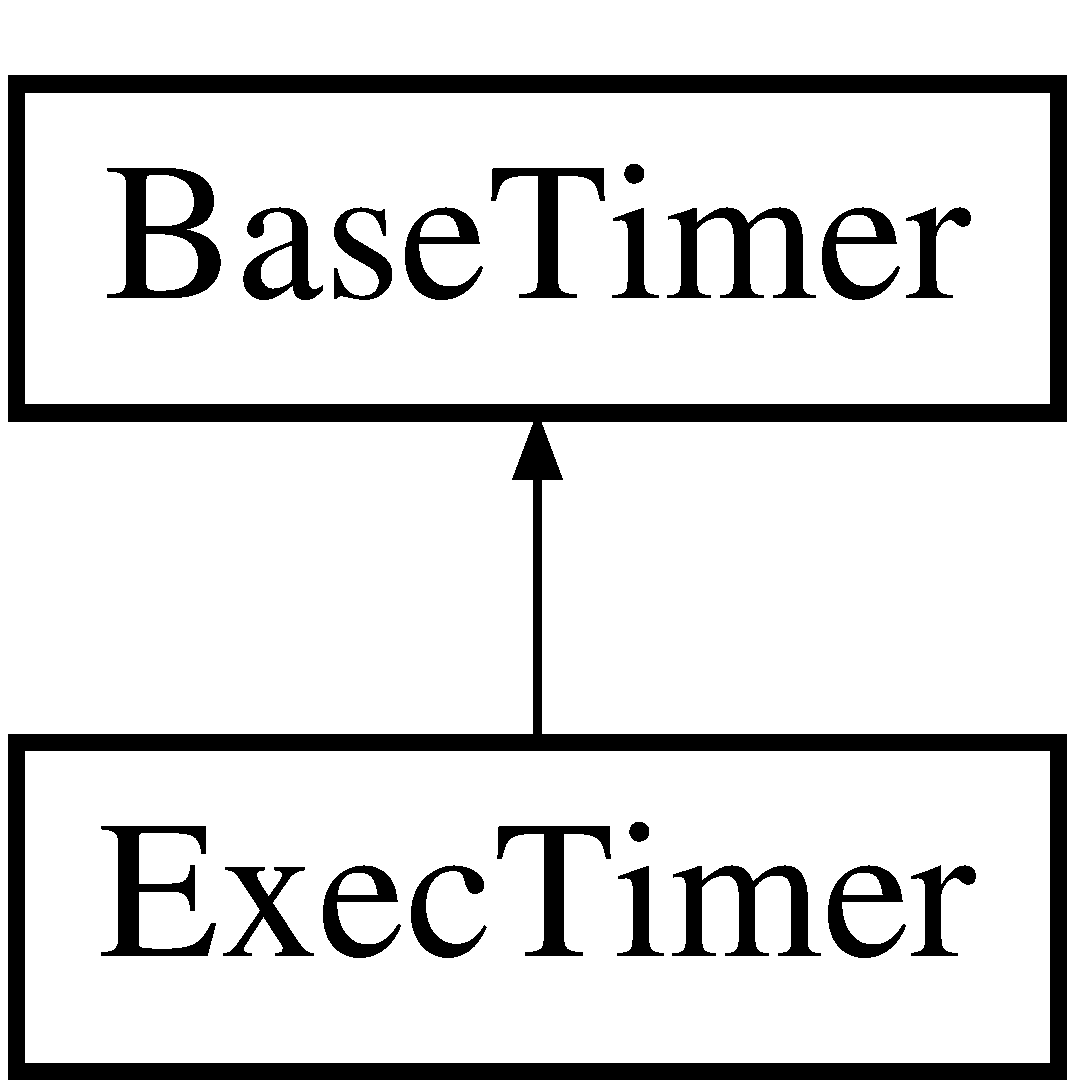
\includegraphics[height=2.000000cm]{class_exec_timer}
\end{center}
\end{figure}
\subsection*{Public Member Functions}
\begin{DoxyCompactItemize}
\item 
\hyperlink{class_exec_timer_a7d5b31a4a84256375e67ab52f943fbd9}{Exec\-Timer} ()
\item 
bool \hyperlink{class_exec_timer_a2ba852cb439905be8e7f4e9cedf753c3}{run} (std\-::string cmd, bool resout)
\end{DoxyCompactItemize}


\subsection{Detailed Description}
This class is used to time a command. The command can be run using the function \hyperlink{class_exec_timer_a2ba852cb439905be8e7f4e9cedf753c3}{run()}. 

\subsection{Constructor \& Destructor Documentation}
\hypertarget{class_exec_timer_a7d5b31a4a84256375e67ab52f943fbd9}{\index{Exec\-Timer@{Exec\-Timer}!Exec\-Timer@{Exec\-Timer}}
\index{Exec\-Timer@{Exec\-Timer}!ExecTimer@{Exec\-Timer}}
\subsubsection[{Exec\-Timer}]{\setlength{\rightskip}{0pt plus 5cm}Exec\-Timer\-::\-Exec\-Timer (
\begin{DoxyParamCaption}
{}
\end{DoxyParamCaption}
)}}\label{class_exec_timer_a7d5b31a4a84256375e67ab52f943fbd9}
The default constructor which initializes everything to zero. 

\subsection{Member Function Documentation}
\hypertarget{class_exec_timer_a2ba852cb439905be8e7f4e9cedf753c3}{\index{Exec\-Timer@{Exec\-Timer}!run@{run}}
\index{run@{run}!ExecTimer@{Exec\-Timer}}
\subsubsection[{run}]{\setlength{\rightskip}{0pt plus 5cm}bool Exec\-Timer\-::run (
\begin{DoxyParamCaption}
\item[{std\-::string}]{cmd, }
\item[{bool}]{resout}
\end{DoxyParamCaption}
)}}\label{class_exec_timer_a2ba852cb439905be8e7f4e9cedf753c3}
This function will time the execution of the command specified in the parameter of this function. This command can contain arguments needed for the execution.


\begin{DoxyParams}{Parameters}
{\em cmd} & The command to be executed. \\
\hline
{\em resout} & A boolean indicating whether or not the results from the command should be printed.\\
\hline
\end{DoxyParams}
\begin{DoxyReturn}{Returns}
True if the program was able to execute, false if the program did not execute properly. 
\end{DoxyReturn}


The documentation for this class was generated from the following files\-:\begin{DoxyCompactItemize}
\item 
Timer/exectimer.\-h\item 
Timer/exectimer.\-cpp\end{DoxyCompactItemize}

%--- End generated contents ---

% Index
\newpage
\phantomsection
\addcontentsline{toc}{chapter}{Index}
\printindex

\end{document}
